\documentclass{beamer}

\usepackage[utf8]{inputenc}

\beamertemplatenavigationsymbolsempty %removes navigation bar

\usepackage{tikz}

\title{Gametic selection, meiotic drive, sex ratio bias, and transitions between sex determination systems}
\author{Michael Scott$^1$, \textbf{Matthew Osmond}$^2$, Sarah Otto$^2$}
\institute{$^1$University College London \& $^2$University of British Columbia}
\date{Evolution 2017}
\titlegraphic{\vspace{1cm}} %lifts text up

\begin{document}

%%%%%%%%%%%%%%%%%%%%%%%%%%%%%%%%%%%%%%%%%%%%%%%%%
%\frame{\titlepage}
\begin{frame}
   \begin{tikzpicture}[overlay, remember picture]
      \node[anchor = south east] at (current page.south east) {
         \includegraphics[width=0.35\textwidth]{IMAGES/Sally}
      };
      \node[anchor = south west] at (current page.south west) {
         \includegraphics[width=0.35\textwidth]{IMAGES/Mike}
      };
   \end{tikzpicture}
      \titlepage
\end{frame}
%%%%%%%%%%%%%%%%%%%%%%%%%%%%%%%%%%%%%%%%%%%%%%%%%

%%%%%%%%%%%%%%%%%%%%%%%%%%%%%%%%%%%%%%%%%%%%%%%%%
\begin{frame}
\frametitle{Sex determination systems are remarkably dynamic}
   \begin{tikzpicture}[overlay, remember picture]
      \node[anchor = center] at (current page.center) {
         \includegraphics[width=\linewidth, angle=0]{IMAGES/TreeOfSex}
      };
      \node[anchor = south east] at (current page.south east) {
         Bachtrog \textit{et al.} 2014
      };
   \end{tikzpicture}
\end{frame}
%%%%%%%%%%%%%%%%%%%%%%%%%%%%%%%%%%%%%%%%%%%%%%%%%

%%%%%%%%%%%%%%%%%%%%%%%%%%%%%%%%%%%%%%%%%%%%%%%%%
\begin{frame}
\frametitle{Turnover can be caused by sex-ratio selection}
   \begin{tikzpicture}[overlay, remember picture]
      \node[anchor = west, text width = 0.5\linewidth] at (current page.west) {
         \includegraphics[width=\linewidth, angle=0]{IMAGES/Hamilton1967Fig1}
      };
      \node[anchor = south west] at (current page.south west) {
         Hamilton 1967
      };
      \node[anchor = east, text width = 0.75\linewidth] at (current page.east) {
         \includegraphics[width=\linewidth, angle=0]{IMAGES/KozielskaEtAl2010Fig1a}
      };
      \node[anchor = south east] at (current page.south east) {
         Kozielska \textit{et al.} 2010
      };
   \end{tikzpicture}
\end{frame}
%%%%%%%%%%%%%%%%%%%%%%%%%%%%%%%%%%%%%%%%%%%%%%%%%

%%%%%%%%%%%%%%%%%%%%%%%%%%%%%%%%%%%%%%%%%%%%%%%%%
\begin{frame}
\frametitle{Turnover can be caused by sex-antagonistic selection}
   \begin{tikzpicture}[overlay, remember picture]
      \node[anchor = center] at (current page.center) {
         \includegraphics[width=0.9\linewidth, angle=0]{IMAGES/vanDoornKirkpatrick2010Fig2}
      };
      \node[anchor = south east] at (current page.south east) {
         van Doorn \& Kirkpatrick 2010
      };
   \end{tikzpicture}
\end{frame}
%%%%%%%%%%%%%%%%%%%%%%%%%%%%%%%%%%%%%%%%%%%%%%%%%

%%%%%%%%%%%%%%%%%%%%%%%%%%%%%%%%%%%%%%%%%%%%%%%%%
\begin{frame}
\frametitle{Haploid selection}
   \begin{tikzpicture}[overlay, remember picture]
      \node[anchor = center] at (current page.center) {
	drive or gametic competition
	- common in plants
	- typically sex-specific
	- inparts both sex ratio and sex-anatagonistic selection
	- outcome for turnover?
      };
   \end{tikzpicture}
\end{frame}
%%%%%%%%%%%%%%%%%%%%%%%%%%%%%%%%%%%%%%%%%%%%%%%%%

%%%%%%%%%%%%%%%%%%%%%%%%%%%%%%%%%%%%%%%%%%%%%%%%%
\begin{frame}
\frametitle{model}
   \begin{tikzpicture}[overlay, remember picture]
      \visible<1->{
         \node[anchor = center, text width = \linewidth] at (current page.center) {
%	    \includegraphics[width=0.4\linewidth, angle=90]{IMAGES/BarfBag1}\\
%	    \includegraphics[width=0.4\linewidth, angle=90]{IMAGES/BarfBag2}
	    \includegraphics[width=0.4\linewidth, angle=0]{IMAGES/BarfBag1}
	    \includegraphics[width=0.4\linewidth, angle=0]{IMAGES/BarfBag2}
	 };
      }  
%      \visible<2->{
%         \node[anchor = east] at (current page.east) {
%	    \includegraphics[width=0.3\linewidth]{IMAGES/LondonBar}
%	};
%      }
   \end{tikzpicture}
\end{frame}
%%%%%%%%%%%%%%%%%%%%%%%%%%%%%%%%%%%%%%%%%%%%%%%%%

%%%%%%%%%%%%%%%%%%%%%%%%%%%%%%%%%%%%%%%%%%%%%%%%%
\begin{frame}
   \begin{tikzpicture}[overlay, remember picture]
      \visible<1->{
         \node[anchor = center, text width = \linewidth] at (current page.center) {
	 \includegraphics[width=\linewidth, angle=0]{../Plots/Combination_Turnover}
	 };
      } 
   \end{tikzpicture}
\end{frame}
%%%%%%%%%%%%%%%%%%%%%%%%%%%%%%%%%%%%%%%%%%%%%%%%%

%%%%%%%%%%%%%%%%%%%%%%%%%%%%%%%%%%%%%%%%%%%%%%%%%
\begin{frame}
   \begin{tikzpicture}[overlay, remember picture]
      \visible<1->{
         \node[anchor = center, text width = \linewidth] at (current page.center) {
	 \includegraphics[width=\linewidth, angle=0]{../Plots/Combination_MeanFit}
	 };
      } 
   \end{tikzpicture}
\end{frame}
%%%%%%%%%%%%%%%%%%%%%%%%%%%%%%%%%%%%%%%%%%%%%%%%%

%%%%%%%%%%%%%%%%%%%%%%%%%%%%%%%%%%%%%%%%%%%%%%%%%
\begin{frame}
   \begin{tikzpicture}[overlay, remember picture]
      \visible<1->{
         \node[anchor = center, text width = \linewidth] at (current page.center) {
	 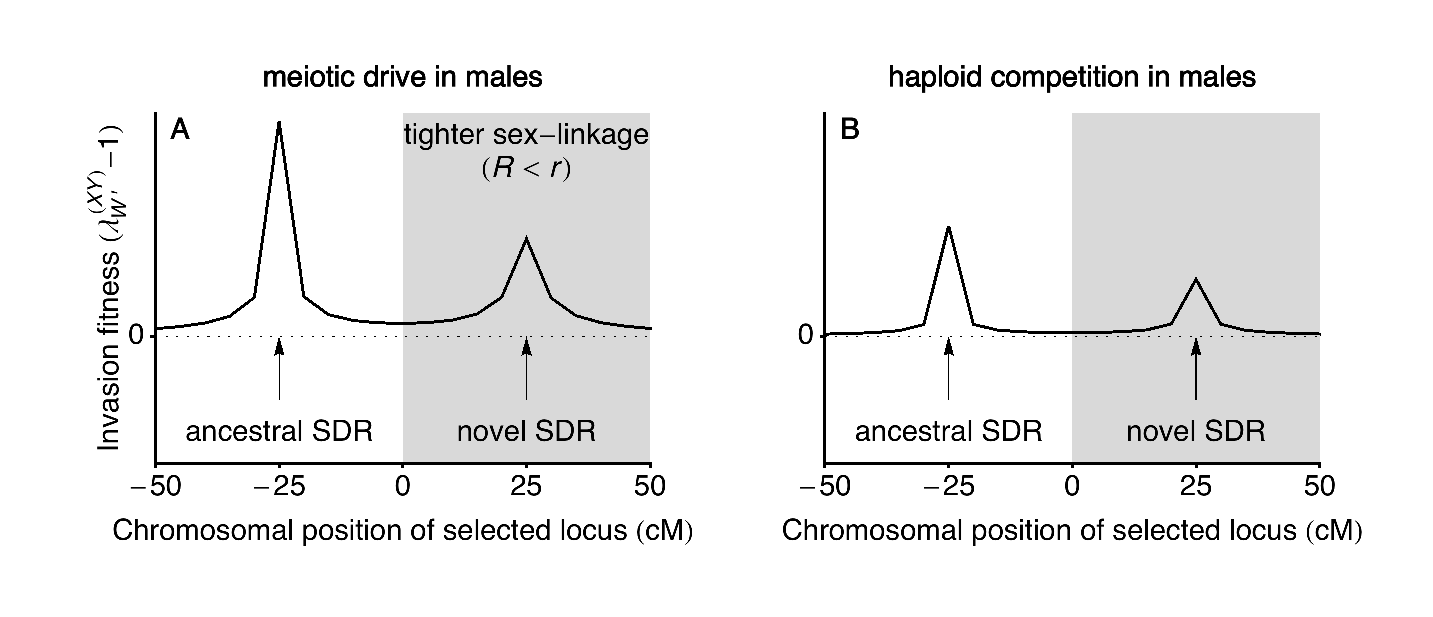
\includegraphics[width=\linewidth, angle=0]{../Plots/PositionPlot}
	 };
      } 
   \end{tikzpicture}
\end{frame}
%%%%%%%%%%%%%%%%%%%%%%%%%%%%%%%%%%%%%%%%%%%%%%%%%

\end{document}